\chapter{Environnement et application}
\label{ch:app}

Nous allons aborder, dans ce chapitre, le nouvel environnement créé a l'aide de Docker et le nouveau code produit à partir de celui de la thèse \thLeite.

L'environnement est réalisé à l'aide de \emph{Docker Compose}, il est composer de trois images différentes. Le code, orienté objet sera executé dans ce nouvel environnement.



\section{Images Docker}
Tous les fichiers necessaire à la construction des images de notre environnement se trouve dans le dossier \emph{$developpement/dockers$}.

\subsection{Hmmer}
La première image est celle visant à remplacer l'utilisation de l'\gls{api} en ligne de HMMER. Il sagit d'encapsuler l'application HMMER afin de pouvoir l'utiliser pour traiter les séquences protéinique.

Les fichiers necessaire se trouvent dans le dossier \emph{$developpement/dockers/hmmer$}. Il sagit d'un image basées sur \emph{centos}, qui est un image de base Docker très legere.

Tout d'abord, le \emph{Dockerfile} de cette image, install le compilateur C++ \emph{gcc}. Puis, il recupere les sources de l'application HMMER et les compilent.

Pour davantage de detail veuillez consulter directement le fichier \emph{Dockerfile} de l'image.

\subsection{Database}
L'application necessite plusieurs base de données Mysql. L'image \emph{database}, dont les sources se trouve dans le dossier \emph{$developpement/dockers/database$}, remplis cette fonctionnalitée.

Pour des raison de simplicité, cette image est construite à partir de Debian Jessie, la différence entre Centos et Debian est négligeable du fait que nous ne lanceront qu'un seul conteneur de cette image.

Due à la fois à la phase de débug et pour de futurs debug, l'image est construite avec un certains nombres de paquets afin de facilité la vie du developpeur.

La mise en place d'une image \emph{Docker} avec un serveur mysql n'est, par experience, jamais une chose facile à réaliser. C'est pour cela que nous allons entré un peu plus dans les détail les différentes commande qui composent le fichier \emph{Dockerfile} de cette image. Il n'est pas forcément necessaire de lire ce sous-chapitre pour comprendre les aboutissant de cette thèse, mais il est necessaire que les informations qui suivent y figure.

Premièrement, afin de pouvoir accèder au conteneur lancé à partir de cette image, il faut faire en sorte que mysql écoute les connexions en entrée.

\lstset{language=bash}
\begin{lstlisting}[frame=single]
RUN sed -i -e"s/^bind-address\s*=\s*127.0.0.1/bind-address = 0.0.0.0/" /etc/mysql/my.cnf
\end{lstlisting}

Maintenant que notre conteneur peut reçevoir des connexions, on install \emph{mysql-server mysql-client libmysqlclient-dev} qui installent Mysql sur notre image.

On peut démarrer le service Mysql:

\begin{lstlisting}[frame=single]
RUN mysqld &
RUN service mysql start
\end{lstlisting}

On oublie pas d'exposer le port de connection que l'on souhaite. Ici le 3306 qui est le port par défault de Mysql.

\begin{lstlisting}[frame=single]
EXPOSE 3306
\end{lstlisting}

On modifie également quelques configuration Mysql, afin de pouvoir utiliser des fichiers \emph{.sql} de tailles plus grandes.

\begin{lstlisting}[frame=single]
RUN sed -ire 's/max_allowed_packet.*=.*/max_allowed_packet = 200M/g' /etc/mysql/my.cnf
RUN sed -ire 's/key_buffer_size.*=.*/key_buffer_size = 128M/g' /etc/mysql/my.cnf
\end{lstlisting}

On ajoute le fichier \emph{startup.sh} et ont fixe qu'au lancement du conteneur il soit executé.

\begin{lstlisting}[frame=single]
ADD ./startup.sh /opt/startup.sh

CMD ["/bin/bash", "/opt/startup.sh"]
\end{lstlisting}

Regardons se que l'on trouve dans le fichier \emph{startup.sh}:

\begin{lstlisting}[frame=single]

if [ ! -f /var/lib/mysql/ibdata1 ]; then

	mysql_install_db

	/usr/bin/mysqld_safe &
	sleep 10s

	echo "GRANT ALL ON *.* TO admin@'%' IDENTIFIED BY 'root' WITH GRANT OPTION; FLUSH PRIVILEGES" | mysql

	# For 1_F1 DetectDomains.py
	echo "CREATE DATABASE phage_bact" | mysql
	mysql phage_bact < /tmp/db/phagesVD.sql
	mysql phage_bact < /tmp/db/bacteriaVD.sql
	mysql phage_bact < /tmp/db/interactionsVD.sql
	mysql phage_bact < /tmp/db/neg_interactionsVD.sql
	mysql phage_bact < /tmp/db/protdom_create.sql
	mysql phage_bact < /tmp/db/progress_create.sql
	mysql phage_bact < /tmp/db/progress_interaction_create.sql

    # For 3_F1 countScoreInteraction.py
	mysql phage_bact < /tmp/db/score_interactions_create.sql

	echo "CREATE DATABASE domine" | mysql
    mysql domine < /tmp/db/domTGo.sql
    mysql domine < /tmp/db/domPfam.sql
    mysql domine < /tmp/db/domPgmap.sql
    mysql domine < /tmp/db/domTInteract.sql

    # For 4_F1 FreqQtdScores.py
	mysql phage_bact < /tmp/db/qtd_scores_create.sql

	killall mysqld
	sleep 10s
fi

/usr/bin/mysqld_safe
\end{lstlisting}

Dans se script, on commence par donner les privilèges Mysql à l'utilisateur admin. Ensuite ont mets en place les différentes base de données, \emph{$phage_bact, domine$}, dont l'application à besoins. On crée ces deux base de données et leurs tables.

Dans l'éventualité ou l'on souhaiterais ajouter une nouvelle base de donnée c'est ici qu'il faudra ajouter la command Mysql de création.

De plus si l'on souaite ajouter des table ou données à une de nos base de données, c'est également dans se fichier qu'il faudra le faire.

Comme vous pouvez le voir tous les fichier \emph{.sql} necessaire sont placé dans le dossier \emph{$developpement/dockers/database/data$}.


\subsection{Core}
%image for bio-info!
Due à la fois à la phase de débug et pour de futurs debug, l'image est construite avec un certains nombres de paquets afin de facilité la vie du developpeur.

C'est véritablemenmt cette images qui contient tous se qui est necessaire à l'execution de l'aspect bioinformatique de l'application. C'est également elle qui controlle l'application, étant donné que cest dans se conteneur que le code de l'application est executé.

Comme pour l'image \emph{database} ont install les paquets necessaire à utiliser Mysql, \emph{mysql-server, mysql-client, libmysqlclient-dev} et python.

On install pip3, le gestionnaire de paquets pip pour python3:

\begin{lstlisting}[frame=single]
RUN apt-get install -y python3-pip r-base
\end{lstlisting}

On install aussi un des paquets les plus important de cestte image.

\begin{lstlisting}[frame=single]
RUN pip3 install biopython
\end{lstlisting}

Afin d'acceder à la base de donnée depuis le code python il nous faut installer le paquet:

\begin{lstlisting}[frame=single]
RUN pip install mysql-connector
\end{lstlisting}

Finalement, on install Docker, car il nous faudra pouvoir communiquer avec l'engin Docker de l'hôte, afin d'executer des conteneur de l'image HMMER.

\begin{lstlisting}[frame=single]
RUN apt-get install -y curl
RUN curl -fsSL https://get.docker.com/ | sh
\end{lstlisting}


\section{Docker Compose}
Maintenant que nous avons toutes les images necessaire à notre environnement applicatif orienté bioinformatique, nous allonms voir comment les combiner à l'aide de \emph{Docker Compose}.

La figure \ref{fig:architecture} montre l'architecture qui est mise en place à l'aide de \emph{Docker}.

\begin{figure}[H] 
\centering 
\includegraphics[width=0.7\columnwidth]{img/architecture} 
\caption[architecture]{Architecture de l'environnement}
\label{fig:architecture} 
\end{figure}

La figure \ref{fig:architecture} montre qu'un conteneur construit à partir de l'image \emph{Core} controllera l'execution du code applicatif et la création de conteneurs basé sur l'image \emph{hmmer}. De plus, tous se qui a trait au donnée stocké en Sql sera géré par le conteneur \emph{Database}.

De cette manière le conteneur \emph{Core} peut créer des conteneurs \emph{hmmer} pour executer les recherche de domaines protéiniques.

Regardons comment cela est mis en place grâce à \emph{Docker Compose}. 

Premièrement, il nous faut un service qui lancera notre conteneur de base de donnée:

\begin{lstlisting}[frame=single]
database:
    build: ../dockers/database
    tty: true
    environment:
      MYSQL_ROOT_PASSWORD: SecretPasswordInphinity
      MYSQL_USER: inphinity
      MYSQL_PASSWORD: SecretPasswordInphinity
      MYSQL_DATABASE: phage_bact
    ports:
      - 3309:3306
    networks:
      mynet:
        ipv4_address: 172.25.0.102
    container_name: inphinity-database
    volumes:
      - /inphinity-data/mysql:/var/lib/mysql
\end{lstlisting}

On specifie que l'on souhaite construire notre conteneur à partir de l'image se trouvant dans le dossier \emph{$/dockers/database$}. En effet, à l'execution de la commande de lancement de notre \emph{compose}, docker compose construira l'image \emph{Database} et créera un conteneur à partir de cette image.

On fixe les paramètres de configuration de Mysql, tel que le mot de passe root, l'utilisateur, sont mot de passe et le nom de la base de donnée par défaut.

On route les ports utile au conteneurs, ainsi que le réseau virtuelle qui sera utilisé.

On fixe manuellement le nom du conteneur qui sera créé afin de facilement pouvoir y acceder en cas de besoins (debug, tests, etc).

Finalement, on ajoute les volumes que l'on souaite à notre conteneur. En effet, avec cette dernière commande, ont attache le dossier hôte \emph{$/inphinity-data/mysql$} au dossier \emph{$/var/lib/mysql$} du conteneur. De cette manière lorsque l'on arrete et relance notre application notre base de donnée ne sera pas détruite. Si l'on souaite supprimer la base de donnée et en recréé une vierge il suffit de supprimer le contenu du dossier \emph{$/inphinity-data/mysql$}.

Deuxièmement, il nous faut un service qui lancera le conteneur de notre contrôleur:

\begin{lstlisting}[frame=single]
core:
    build: ../dockers/core
    hostname: core
    networks:
      mynet:
        ipv4_address: 172.25.0.101
    tty: true
    volumes:
      - ../inphinity:/inphinity:Z
      - ../dockers/core/data-hmm:/data-hmm:Z
      - /var/run/docker.sock:/var/run/docker.sock
    privileged: true
    links:
      - database:database
    depends_on:
      - database
    container_name: inphinity-core
\end{lstlisting}

On suit exactement la même logique que pour notre premier service. On specifie que l'on souhaite construire notre conteneur à partir de l'image se trouvant dans le dossier \emph{$/dockers/core$}. En effet, à l'execution de la commande de lancement de notre \emph{compose}, docker compose construira l'image \emph{COre} et créera un conteneur à partir de cette image.

On attribue le réseau virtuelle qui sera utilisé, le même que pour le service de la base de donnée.

On fixe manuellement le nom du conteneur qui sera créé, afin de facilement pouvoir y acceder en cas de besoins (debug, tests, etc).

On ajoute les volumes necessaire:

\begin{itemize}
\item ../inphinity:/inphinity, contient le code applicatif;
\item ../dockers/core/data-hmm:/data-hmm, servira à transmettre les fichiers de résultats des analyses réalisé par les conteneurs hmmer au contrôleur;
\item /var/run/docker.sock:/var/run/docker.sock, permet au controleur de communiquer avec l'engin Docker de l'hôte et donc de créer les conteneur hmmer à la volée.
\end{itemize}

On lie, grâce à la commande \emph{links}, le contôleur à la base de données.

La copmmande \emph{$depends_on$} permet de garantir que le conteneur "core" sera crée uniquement après la création du conteneur "database".

Le troisième service se trouvant le le fichier compose n'est pas necessaire car on lancéra les conteneur hmmer directement depuis le code python de notre application. 

Finalement, on définit un réseau dans lequel on place les conteneur de l'application.

\section{<<Inphinity Environment>>}

Comme déjà précisé précédement, une première optimisation du code est passé par le fait de traduire les code existant du python2 vers le python3.3 .

Au niveau du code, la logique suivie à été de diviser le code en \emph{phases} successives. Chacune de ces phases est chargées d'un traitement spécifique, de remplir un objectif.

Attention, ce chapitre n'aborde pas la logique du code réalisé dans la thèse \thLeite , il n'est question ici que de la plusvalue ajouté lors de se travail de master.

Les fonction utilisées dans les script de la thède \thLeite reste très proche de celle de se travail!

\subsection{Diagramme de classes}
\begin{figure}[H] 
\centering 
\includegraphics[width=1\columnwidth]{img/class_diagram} 
\caption[classdiagram]{Diagramme de classes}
\label{fig:classdiagram} 
\end{figure}

\subsubsection{Core}
La classe \emph{Core} est la classe principal de l'application. C'est elle qui est chargée d'instancier les classe neccessaire au bon déroulement du code et de lancer les phase du processus.

Comme ont le voit sur la figure \ref{fig:classdiagram}, la classe \emph{Core} possède une instance des cinq classes, représentant chacune une phase du processus. Elle possède également une instance de la classe \emph{Tools}, qui donne accès a l'objet de la classe \emph{Config}, gerant le \emph{parsing} de la configuration en cours. De plus, la classe \emph{Tools} possède un acces à l'objet \emph{DBUtilities}, qui gère l'ensemble des accès aux base de données.

\subsubsection{Phase 1 - DetectDomaines}

C'est durant cette phase que l'utilisation à HMMER est faite, c'est dans cette phase que la parallélisation de cette utilisation est réalisée. Plus précisément regardons la fonction \emph{$seek_domaines_multiprocess()$}, on y initialise une \emph{Multiprocessing.Pool} avec un certain nombre de coeurs à disposition. Ce nombre de coeurs est définit dans les fichiers de configuration, cf. \ref{ch:config}.

Ensuite, on divise le tableau des séquence à traité en \emph{chunk}, cela permet d'obtenir les résultats également par series de 'n' réponse et de les incerer dans la base de donnée au fur et à mesure. Cela afin d'éviter de perdre du temps d'analyse en cas d'arrète de l'application.

\lstset{language=python}
\begin{lstlisting}[frame=single]
chunk_size = pool_size * self.tools.configuration.get_chunk_size_multiplier()
        chunks = self.chunks(list(tab), chunk_size)
\end{lstlisting} 

Lorsque l'on insert les résultats dans la base de donnée ont inssert également dans la table \emph{progress} qu'elle séquences ont été analysé. Cela nous permet d'arreter et de relancer l'application quand ont veut sans pour autant devoir recommencer la phase d'analyse a zéro.

Ont execute le code suivant pour chacun des \emph{chunks}:
\begin{lstlisting}[frame=single]
for chunk in chunks:
            print('%d sequences processed!' % total_processed)
            LOGGER.log_normal('%d sequences processed!' % total_processed)
            total_processed += chunk_size
            results = p.map(self.hmmer_scan.analyze_domaines, chunk)
            print(results)

            for prot in chunk:
                self.tools.db.analyze_done(prot[0], 1)

            for result in results:
                try:
                    id_prot = result[0]
                    domaines_returned = result[1]

                    self.tools.db.execute_insert_domains(id_prot, domaines_returned, id_cell, bool_bacteria, "--")
\end{lstlisting} 

On fait appelle de manière parallel à la fonction \emph{$hmmerScan.analyze_domaines()$}. Grâce à la \emph{pool} de processus la fonction sera executée simultanément un certain nombre de fois.

Allons voir plus en détail se qui se passe dans cette fonction. Pour voir le code de la fonction en détail, veuillez vous rendre directement dans les sources du code (\emph{$developpement/inphinity/v_0.5/hmmerScan.py$}).

La séquence envoyé à la fonction est \emph{parsé} dans un fichier temporaire:

\begin{lstlisting}[frame=single]
fasta = '>' + values_tab[0] + '\n' + values_tab[1] + '\n'
fasta_filename = '/data-hmm/tmp/' + str(uuid.uuid4()) + '.fasta'
self.io.write(fasta_filename, fasta)
\end{lstlisting} 

On crée également un fichiers temporaire ou sera stoqué le résultats de l'analyse par \emph{HMMER scan}:

\begin{lstlisting}[frame=single]
results_filename = "/data-hmm/results/hits_test_" + str(uuid.uuid4()) + ".txt"
\end{lstlisting} 

Par la suite le code fait appele à la fonction \emph{Subprocess.Popen()} permettant de réaliser de commande UNIX directement depuis un code python. Grâce à cela on peu lancer une commande qui créera un nouveau conteneur Docker qui effectuera une analyse de séquence, Une fois l'analyse effectuée le conteneur s'arrete automatiquement.


\begin{lstlisting}[frame=single]
p = subprocess.Popen([
                "docker " +
                "run " +
                "--rm " +
                "--privileged " +
                "-v " +
                path_to_core + "/data-hmm:/data-hmm " +
                "inphinity-hmmer " +
                "hmmsearch " +
                "--tblout " +
                results_filename + " " +
                "/data-hmm/Pfam-A.hmm " +
                fasta_filename
            ], stdout=subprocess.PIPE, shell=True)

            (output, err) = p.communicate()

            # This makes the wait possible
            p_status = p.wait()
\end{lstlisting} 

Cette commande lance un conteneur docker avec l'image que l'on à préalablement créée pour encapsuler HMMER. On spécifie le fichier dans lequel se trouve la séquence au format \emph{FASTA}, ainsi que le fichier dans lequel oont souhaite inscrire les résultats de l'analyse.

Ensuite, on lit, récupere et filtre les résultats:

\begin{lstlisting}[frame=single]
results = self.io.read_results(results_filename, self.configuration.get_detailed_logs())

[...]
\end{lstlisting}

Nous aborderont la selection des résultats dans la section \ref{ch:config}.

Finalement on supprime les deux fichiers temporaire et ont retourne les résultats.

\begin{lstlisting}[frame=single]
p = subprocess.Popen([
	"rm",
	results_filename
 ])
 p.communicate()
 p_status = p.wait()

 p = subprocess.Popen([
 	"rm",
 	fasta_filename
 ])
 p.communicate()
 p_status = p.wait()

return [values_tab[0], returned_domains, [start_time, end_time]]
\end{lstlisting}

\subsection{Configuration}
\label{ch:config}

Toutes les interactions utilisateurs que les scripts produit lors de la thèse \thLeite ont été remplacé par une valeur dans le fichier de configuration.

\subsubsection{Lancement des configurations}

La classe \emph{Main} de l'application (app.py) est fait pour lancer la fonction \emph{$Core.run()$} pour chaque fichier de configuration se trouvant dans le dossier \emph{$inphinity/v_0.5/configs$}. Il faut préciser que seule les fichier finissant par l'extension \emph{.ini} sont considéré comme des fichier de configuration. Donc pour garder une configuration, tout en empechant quelle soit utilisée, il suffit d'ajouter \emph{.old} à la fin, par exemple.

\begin{lstlisting}[frame=single]
if __name__ == '__main__':
    os.chdir("inphinity/v_0.5/configs")
    configs = glob.glob("*.ini")

    for config_file in configs:
        print('Config file: %s' % config_file)

        c = Core(config_file)
        c.run()
\end{lstlisting}

Voici, un fichier de configuration standard:

\begin{lstlisting}[frame=single]
[INFORMATION]
verbose = 0
detailed_logs = 0
testing = 0
[ENV]
path_to_core = /home/kamyh/projects/master/developpement/dockers/core
#Dile to parse sequences
temp_file_pseqs = /tmp/tmpMF.txt
reset_db_at_start = 0
#if = 0 --> auto
#if = -1 --> nbr of core
#if = x --> x
process = -1
# Smaller the chunk are, the more time is lost
chunk_size_multiplier = 4
phases_to_run = 1,2,3,4,5
[PHASE_1]
analyze_phage = 1
analyze_bacteria = 1
[DOMS_SELECTION]
use_e_value_selection = 0
min_e_value = 9.8e-25
max_e_value = 1500

use_score_selection = 0
min_score = 0
max_score = 1500

use_biais_selection = 0
min_biais = 0
max_biais = 1500
[DATASET_GENERATION]
grades_file_pseqs = /inphinity/grades/gradesDict.p
ds_dir = /inphinity/datasets/
normalisation = 0
# 1 --> Number of bins
# 2 --> Vector of bins
type_bins = 1
number_of_bins = 1
space_between_bins = 1
\end{lstlisting}

Etant donné l'importance des fichiers de configuration dans la productions de dataset interessants, nous allons passer en revu les différents éléments y etant définit.

Premièrement, il faut savoir que l'on trouve deux type d'élément dans un fichier de configuration, des sections et de valeurs. Les section sont des mots clés entre crochets, eg. [INFORMATION], et en majuscules. Les valeurs sont en minuscules, et se rapport chacune à une section. En effet, toutes les valeurs àprès une section, font partie de cette section. Cela permet d'organiser le fichier de configuration au mieux.

\textbf{Section - [INFORMATION]}

Ces valeurs de configuration servent lors des phase de développement et tests.

\begin{itemize}
\item \emph{verbose}, permet de désactiver la pluspart de affichage console.
\item \emph{$detailed\_logs$}, permet d'inscrire dans les logs des information détaillées sur l'execution de l'application.
\item \emph{testing}, permet de limiter le nombre d'organisme traité par l'application, à des fin de développement ou de tests. 
\end{itemize}

\textbf{Section - [ENV]}

Les configurations se trouvant sous cette section concerne des variable d'environnement de l'application.

\begin{itemize}
\item \emph{$path\_to\_core$}, afin de fonctionne, l'application, à besoins de connaitre l'emplacement du dossier contenant la description Docker de l'image du contrôleur principal.
\item \emph{$temp\_file\_pseqs$}, permet de spécifier le fichiers temporaire qui sera utilisé afin de parser les sequences multi-fasta. 
\item \emph{$reset\_db\_at\_start$}, permet de réinitialiser la base de donnée au lancement de l'application.
\item \emph{process}, spécifie le nombre de coeurs qui sera alloué à la \emph{pool}. 
\begin{itemize}
\item fixé à "0", laisse la librairie automatiquement définir le nombre de coeur, normalement le nombre maximum disponnible.
\item fixé à "-1", fixe le nombre de coeur au maximum disponnible moins 1. Cette méthode permet de laisser un coeur libre pour les processus de la mchine hôte.
\item fixé à "x", laisse choisir le nombre de coeurs, mais attention en mettre davantage que le maximum ralentit l'execution de l'application.
\end{itemize}
\item \emph{$chunk\_size\_multiplier$}, définit la taille de \emph{chunk} pour le traitement des séquence lors de la phase 1.
\item \emph{$phases\_to\_run$}, permet de définir quelles phases ont souhaite executer. Par exemple, si la valeur est égale à "1,2,3,4,5", toutes les phases seront executée. On peut choisir de n'executer que les deux derniere phase en inscrivant la valeur de se parametre à "4,5".
\end{itemize}

\textbf{Section - [$PHASE_1$]}

Configurations se rapportant directement à l'execution de la phase 1 du traitement.

\begin{itemize}
\item \emph{$analyze\_phage$}, permet de définir si les phages doivent etres traités.
\item \emph{$analyze\_bacteria$}, permet de définir si les bacteries doivent etres traités.
\end{itemize}

\textbf{Section - [$DOMS\_SELECTION$]}

Une analyse de séquence par \emph{hmmsearch} donne des résultats semblable à la figure \ref{fig:hmmseach}. On voit que chaque domaines trouvé possède une valeure de score, une e-value et un biais.

\begin{figure}[H] 
\centering 
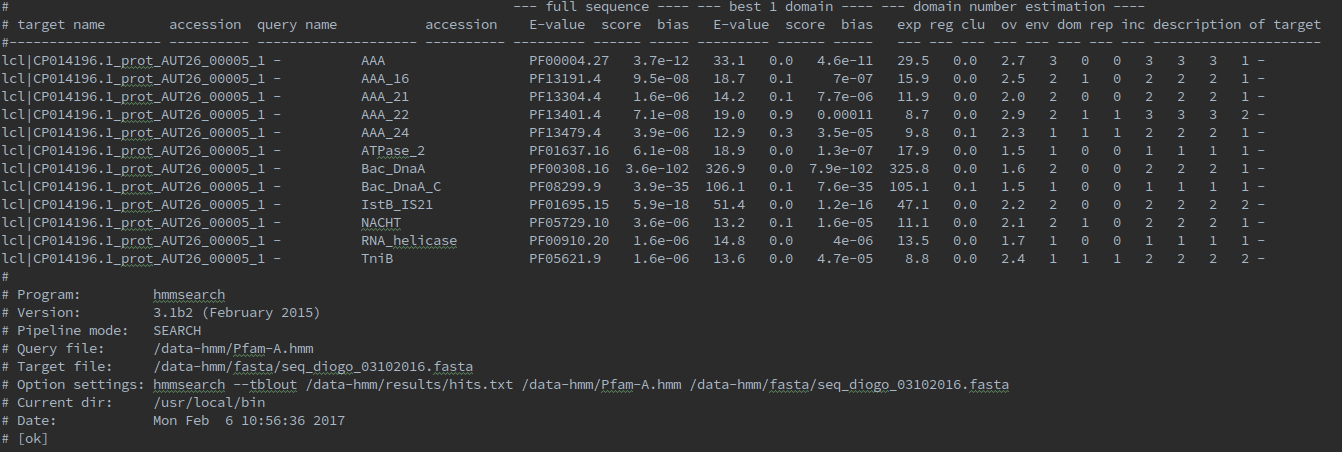
\includegraphics[width=1\columnwidth]{img/hmmsearchresult} 
\caption[hmmseach]{Résultats de hmmerseach}
\label{fig:hmmseach} 
\end{figure}

\begin{itemize}
\item \emph{$use\_e\_value\_selection$}, \emph{$min\_e\_value$}, \emph{$max\_e\_value$}, ces trois valeurs permet de filtré la selection des résultats de l'analyse HMMER en utilisant la \emph{e-value}.
\item \emph{$use\_score\_selection$}, \emph{$min\_score$}, \emph{$max\_score$}, ces trois valeurs permet de filtré la selection des résultats de l'analyse HMMER en utilisant le \emph{score}.
\item \emph{$use\_biais\_selection$}, \emph{$min\_biais$}, \emph{$max\_biais$}, ces trois valeurs permet de filtré la selection des résultats de l'analyse HMMER en utilisant la valeure de  \emph{biais}.
\end{itemize}

\textbf{Section - [$DATASET_GENERATION$]}

\begin{itemize}
\item \emph{$grades\_file\_pseqs$}, emplacements du dictionnaire des score pour la création du dataset.
\item \emph{$ds\_dir$}, emplacement du dossier dans lequel placer le dataset créé. Le nom du dataset est définit en ajoutant au nom de la configuration la date et l'heure.
\item \emph{normalisation}, spécifie si les valeurs du datasets doivent etre normalisé.
\item \emph{$type\_bins$}, selectionne quell type de bins contient le dataset produit.
\begin{itemize}
\item fixé à "1", siginfie que l'on souhaite spécifier le nombre de \emph{bins} à produire.
\item fixé à "2", signifie que l'on souhaite un vecteur de \emph{bins}.
\end{itemize}
\item \emph{$number\_of\_bins$}, permet de définir le nombre de \emph{bins}.
\item \emph{$space\_between\_bins$}, permet de définir l'espacement entre les \emph{bins}.
\end{itemize}

\subsection{Loggs}
Afin de facilité le développement de se travail et les futurs développement et modification de l'application, une classe permettant la génération d'un fichiers de \emph{log} (compte-rendu). COmme on le voit sur la figure \ref{fig:classdiagram}, il y a cinq niveau de \emph{log}. Cela permet d'organiser les information que l'on souhaite enregistrer.

Chacun des niveau de \emph{log} possède un mot clé qui est placé au début de la ligne du message dans le fichier compte-rendu.

\lstset{language=bash}
\begin{lstlisting}[frame=single]
DETAILS 2017-01-22 12:35:18| <<very detailed message!>>
DETAILS 2017-01-22 12:35:34| <<very detailed message!>>
DETAILS 2017-01-22 12:35:56| <<very detailed message!>>
ERROR 2017-01-22 12:36:18| <<error message!>>
DEBUG 2017-01-22 12:37:18| <<debug message!>>
DEBUG 2017-01-22 12:37:19| <<debug message!>>
DEBUG 2017-01-22 12:37:20| <<debug message!>>
DEBUG 2017-01-22 12:37:21| <<debug message!>>
DEBUG 2017-01-22 12:37:22| <<debug message!>>
DEBUG 2017-01-22 12:37:23| <<debug message!>>
\end{lstlisting}

Grâce au mots clé en début de ligne, il est très facile de consulter les \emph{logs} au niveau de l'on souhaite. La commande suivante, permet d'obtenir les 1000 dernière lignes contenant le mots "NORMAL":

\begin{lstlisting}[frame=single]
$ tail -1000 /tmp/logs_inphinity.txt |grep NORMAL
\end{lstlisting}













































